\section{Dataset Similarity and Synthetic-Data Fidelity}
\label{sec:similarity-fidelity}

\subsection{Purpose and analysis framework}

The two TabPFN transformations require different forms of evaluation.  An
embedding contains the original patients represented by new numerical
coordinates, so the relevant question is whether relationships among those
patients are retained.  A synthetic cohort contains newly generated records in
the original clinical format, so it can be compared with the real cohort in
terms of distributions, clinical subgroups, survival patterns and fitted-model
behaviour.  No single similarity score can answer all of these questions.

Table~\ref{tab:fidelity:framework} summarises the four complementary analyses.
All synthetic-data results describe one generated diagnostic cohort and one
generated prognostic cohort, each produced by a generator trained on the
corresponding complete real cohort.  The results do not include variation from
retraining the generator or sampling additional synthetic cohorts, and they do
not constitute external validation.

\begin{table}[htbp]
\centering\small
\caption{Questions addressed by the similarity and fidelity analyses.}
\label{tab:fidelity:framework}
\begin{tabularx}{\linewidth}{@{}>{\RaggedRight\arraybackslash}p{2.15cm}
>{\RaggedRight\arraybackslash}p{2.65cm}YY@{}}
\toprule
Analysis & Data compared & Main measures & Interpretation \\
\midrule
Embedding structure & Clinical and embedding representations of the same
patients & Trustworthiness, continuity and Mantel correlation & Preservation of
local neighbours and overall distance ordering \\
Synthetic distribution & Real and generated records containing predictors and
outcomes & Marginal differences, discriminator tests, correlation differences
and nearest-record distance & Statistical differences detectable under the
specified preprocessing and models \\
Clinical structure & Real and generated categories, subgroups, outcomes and
survival curves & Category support, subgroup outcomes, survival differences and
adjusted relationships & Clinical patterns that appear preserved, distorted or
unavailable in the generated cohorts \\
Model portability & Identically specified models trained on real or generated
records and scored on the real source cohort & Discrimination differences and
coefficient-sign agreement & Compatibility within the source cohort, not
independent generalisation \\
\bottomrule
\end{tabularx}
\end{table}
\FloatBarrier

\subsection{Preservation of embedding structure}
\label{sec:fidelity:embedding}

Trustworthiness measures whether patients who are close in an embedding were
also close in the clinical representation; it penalises new neighbours created
by the transformation.  Continuity measures whether clinically similar patients
remain neighbours after transformation.  Both metrics range from zero to one,
with one indicating perfect neighbourhood preservation
\citep{Venna2001}.  Results were calculated for neighbourhoods of 10 and 30
patients.

The Mantel analysis compares the ordering of all pairwise patient distances in
the two representations using a Spearman correlation
\citep{Mantel1967}.  Significance was assessed with 499 permutations of patient
labels.  For every embedding block, none of the permuted correlations was as
large as the observed value; the resulting value of 0.002 is the smallest
permutation probability available with this number of permutations.

The diagnostic embedding preserved local structure most strongly, with
trustworthiness of 0.953 and continuity of 0.952 for 10-neighbour sets
(Table~\ref{tab:fidelity:embedding}).  Its Mantel correlation was 0.558,
indicating moderate preservation of overall distance ordering.  The prognostic
event and follow-up-time blocks showed weaker local and global preservation.
Combining the two prognostic blocks improved continuity and the Mantel
correlation relative to either block alone, but remained below the diagnostic
embedding.

\begin{table}[htbp]
\centering\scriptsize
\caption{Structural preservation between the clinical representation and each
TabPFN embedding.  Every row uses all matched patients.}
\label{tab:fidelity:embedding}
\begin{tabularx}{\linewidth}{@{}Yrrrrrrr@{}}
\toprule
Embedding block & $n$ & \shortstack{Trust\\$k=10$} &
\shortstack{Continuity\\$k=10$} & \shortstack{Trust\\$k=30$} &
\shortstack{Continuity\\$k=30$} & Mantel $r$ & $p$ \\
\midrule
\csname @@input\endcsname{tables/similarity_fidelity/embedding_structure_rows.tex}
\bottomrule
\end{tabularx}
\end{table}

\begin{figure}[htbp]
\centering
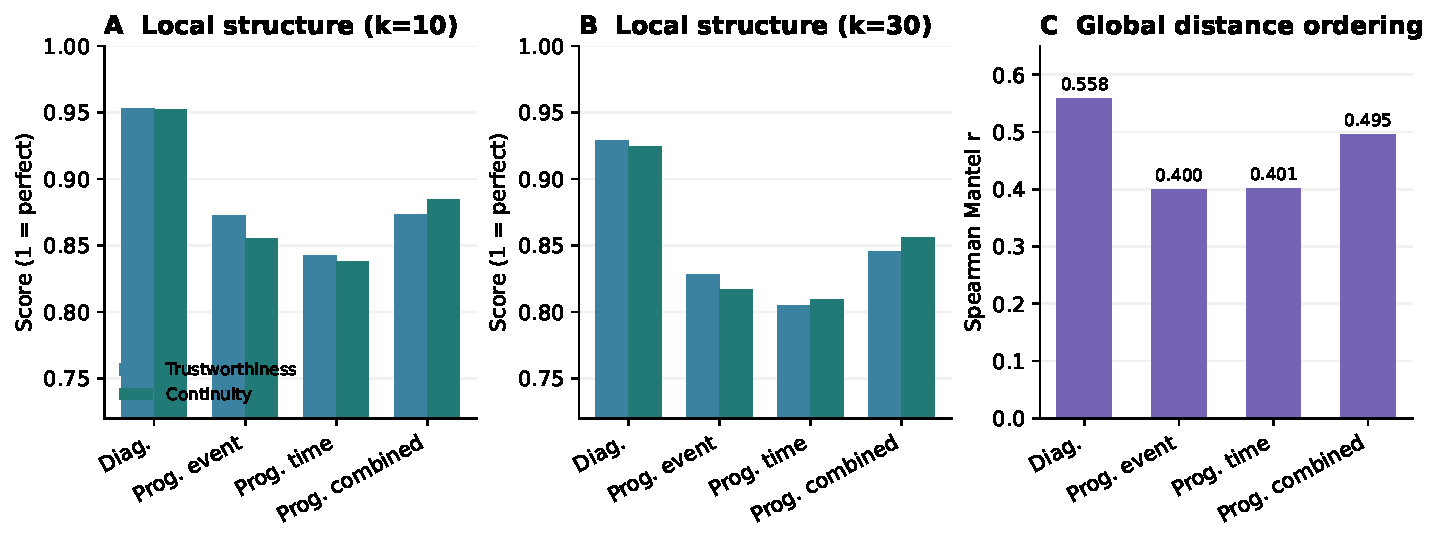
\includegraphics[width=\linewidth]{similarity_fidelity/embedding_structure_summary.pdf}
\caption{Local-neighbourhood preservation and overall distance-order
preservation for the diagnostic and prognostic embeddings.  These metrics
describe representation structure, not predictive performance.}
\label{fig:fidelity:embedding}
\end{figure}
\FloatBarrier

Two design choices are important when interpreting these results.  First, the
clinical representation used for the distance calculations includes the
liver-metastasis outcome for diagnosis and both death status and follow-up time
for prognosis.  Because the embeddings were also supervised using these
outcomes, the results describe preservation of outcome-inclusive clinical
structure rather than predictor-only structure.  Second, nominal categories
were converted to numerical codes before standardised Euclidean distances were
calculated.  This imposes an artificial ordering on categories such as race and
histology.  The scores are therefore useful within this specified encoding but
are not encoding-independent properties of the data.

Figure~\ref{fig:fidelity:diagnostic-tsne} provides a complementary qualitative
view using t-distributed stochastic neighbour embedding (t-SNE). Each panel was
fitted independently in its own feature space: Gower distances \citep{Gower1971} were used for
the real and synthetic clinical data, while standardised Euclidean distances
were used for the dense TabPFN coordinates. The axes and cluster locations
therefore cannot be compared directly across panels.

\begin{figure}[htbp]
\centering
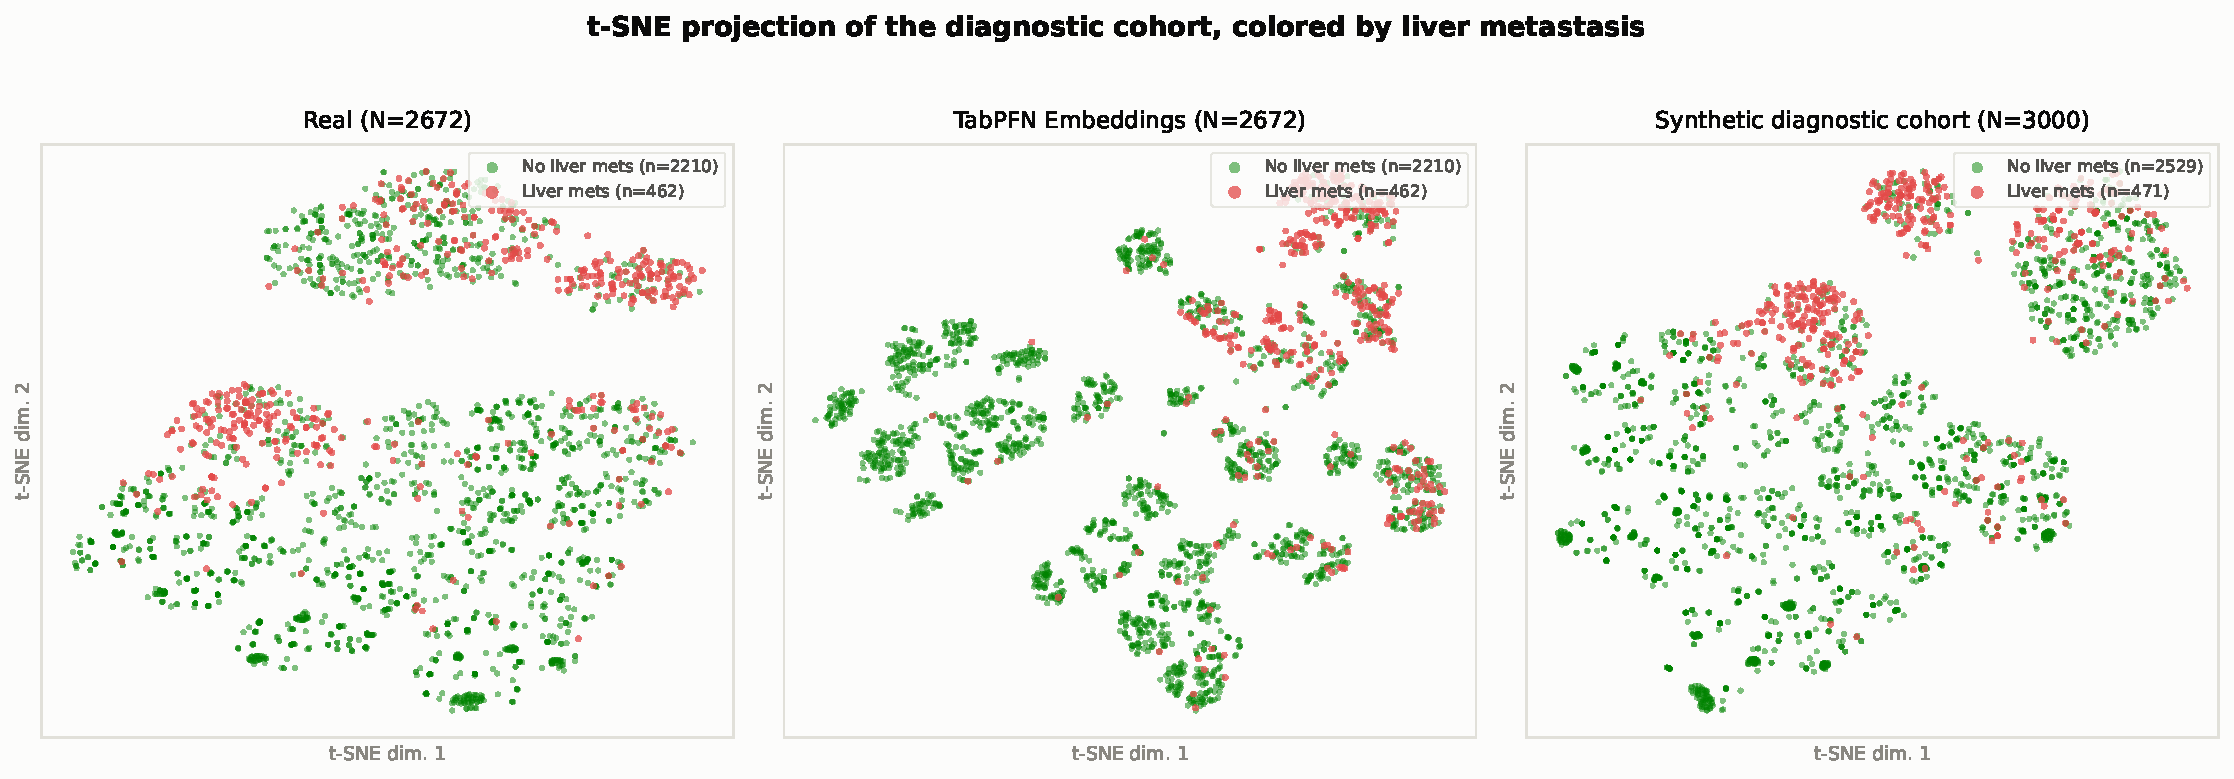
\includegraphics[width=\linewidth]{similarity_fidelity/diagnostic_tsne_panels.pdf}
\caption{Independent t-SNE projections of the real diagnostic clinical space,
the TabPFN embedding and the complete synthetic diagnostic cohort. Points are
coloured by liver-metastasis status. The panels show local organisation within
each representation; their coordinates do not form a shared space.}
\label{fig:fidelity:diagnostic-tsne}
\end{figure}

All three projections contain outcome-related local grouping together with
substantial overlap between patients with and without liver metastasis. The
embedding forms more compact local clusters, which is consistent with its high
neighbourhood-preservation scores. The synthetic projection recreates broad
outcome-associated grouping, but its cluster shapes and densities differ from
the real clinical projection. Because t-SNE emphasises local neighbourhoods and
can alter global geometry, the figure supports only a qualitative description;
it does not establish distributional fidelity or performance in new patients.
\FloatBarrier

\subsection{Overall similarity of the synthetic cohorts}
\label{sec:fidelity:synthetic-distribution}

Two discriminator-based tests assessed whether real and synthetic records could
be distinguished when predictors and outcomes were considered together.
Nominal variables were represented by separate indicator columns, continuous
variables were standardised and binary or ordinal variables were entered
numerically.

The propensity-score mean squared error (pMSE) ratio compares the separation
achieved by an in-sample logistic discriminator with the separation expected if
real and synthetic records came from the same distribution
\citep{Snoke2018}.  A ratio near one indicates little detectable separation
under this model.  The classifier two-sample test (C2ST) uses five-fold
out-of-fold logistic predictions; its area under the receiver operating
characteristic curve (AUC) is expected to be 0.5 when the datasets cannot be
distinguished \citep{LopezPaz2017}.

Both synthetic cohorts were distinguishable from their real counterparts
(Table~\ref{tab:fidelity:synthetic-global}).  The C2ST AUC was 0.630 for
diagnosis and 0.664 for prognosis, while the pMSE ratios were 31.748 and 9.500.
The pMSE ratios should not be ranked across tasks because their reference values
depend on sample size and the number of discriminator variables.

\begin{table}[htbp]
\centering\scriptsize
\caption{Overall real-versus-synthetic distribution checks.  Correlation
differences are absolute differences between Pearson-correlation matrices over
numeric, binary and ordinal fields.  Nearest-record distances use min--max
scaled variables and numerical category codes, so their magnitudes are not
comparable across tasks.}
\label{tab:fidelity:synthetic-global}
\begin{tabularx}{\linewidth}{@{}>{\RaggedRight\arraybackslash}p{1.4cm}
*{6}{>{\centering\arraybackslash}X}@{}}
\toprule
Task & pMSE ratio & C2ST AUC & Mean correlation difference &
Maximum correlation difference & Median nearest-real distance & Exact real-row matches \\
\midrule
\csname @@input\endcsname{tables/similarity_fidelity/synthetic_similarity_rows.tex}
\bottomrule
\end{tabularx}
\end{table}

Average pairwise correlations were similar, with mean absolute differences of
0.018 for diagnosis and 0.045 for prognosis.  The largest correlation
differences were 0.084 and 0.154, showing that average agreement can conceal
larger discrepancies for individual variable pairs.

Most continuous-variable distributions were also close.  The Wasserstein
distance for age was 0.024 diagnostic interquartile ranges (IQRs) in the
diagnostic cohort and 0.049 IQRs in the prognostic cohort.  For tumour size, the
corresponding values were 0.026 and 0.084 IQRs.  The diagnostic tumour-size
Kolmogorov--Smirnov test gave \(p=0.044\), but this was one of many unadjusted
marginal tests and is not interpreted as an isolated finding.

No synthetic record exactly matched a complete real record.  This is a useful
basic check, but it does not demonstrate privacy.  The nearest-record distance
depends on cohort size, dimensionality and the numerical coding of nominal
categories, and neither membership-inference risk nor a formal
differential-privacy guarantee was evaluated.

\subsection{Grade and subgroup preservation}

Histological grade was the clearest marginal distortion
(Table~\ref{tab:fidelity:grade}).  In the diagnostic cohort, grade I increased
from 71.7\% of real patients to 93.2\% of synthetic records, while grades II
and III decreased from 19.7\% and 6.3\% to 4.9\% and 1.9\%.  All 60 real
grade-IV patients were absent from the synthetic cohort.  In the prognostic
cohort, grade I increased from 44.4\% to 72.1\%, grade III decreased from
20.8\% to 7.1\%, and all 33 grade-IV patients were absent.  The generator also
failed to reproduce the single diagnostic patient recorded with Goblet-cell
carcinoid histology.

\begin{table}[htbp]
\centering\small
\caption{Histological-grade representation in the real and synthetic cohorts.
The distortion categories use the predefined relative-share thresholds:
moderate for changes of at least 25\% and high for changes of at least 50\%.
Lost indicates that a real category is absent from the synthetic cohort.}
\label{tab:fidelity:grade}
\begin{tabularx}{\linewidth}{@{}YcrrrrY@{}}
\toprule
Task & Grade & Real ($n$) & Synthetic ($n$) & Real \% & Synthetic \% &
Distortion category \\
\midrule
\csname @@input\endcsname{tables/similarity_fidelity/grade_preservation_rows.tex}
\bottomrule
\end{tabularx}
\end{table}

The relationships between grade and outcome also changed.  Among diagnostic
grade-II records, liver-metastasis prevalence increased from 0.243 in the real
cohort to 0.592 in the synthetic cohort.  For grade III, it increased from
0.571 to 0.724.  In the prognostic grade-II subgroup, mortality increased from
0.672 to 0.875 and median observed follow-up or death time decreased from 48 to
21.5 months.  These are descriptive differences between cohorts, not causal
effects of grade.  Because grade IV is completely absent, its outcome
relationships cannot be evaluated in either synthetic cohort.

\subsection{Survival-curve fidelity}

Kaplan--Meier survival estimates were compared between the 462 real and 462
synthetic prognostic records.  Each cohort contained 311 observed deaths.
Synthetic survival was higher by 0.057 at 12 months, 0.030 at 24 months and
0.053 at 36 months (Table~\ref{tab:fidelity:survival}).  Restricted mean
survival time (RMST) through 36 months was 1.55 months longer in the synthetic
cohort.

\begin{table}[htbp]
\centering\small
\caption{Overall Kaplan--Meier survival and 36-month restricted mean survival
time in the real and synthetic prognostic cohorts.  Differences are synthetic
minus real.}
\label{tab:fidelity:survival}
\begin{tabular}{@{}lrrr@{}}
\toprule
Horizon or summary & Real & Synthetic & Difference \\
\midrule
\csname @@input\endcsname{tables/similarity_fidelity/survival_preservation_rows.tex}
\bottomrule
\end{tabular}
\end{table}

The overall two-sample log-rank test gave \(p=0.315\).  This failure to detect a
difference is not evidence that the curves are equivalent.  The generated
cohort was learned from the real cohort, and the analysis does not include
uncertainty from repeating generation.

Subgroup comparisons revealed larger differences than the overall curve.  The
largest survival-probability difference across 12, 24 and 36 months was 0.310
for grade II, 0.233 for patients with bone metastasis and 0.200 for patients
with lung metastasis.  A difference of 0.667 for T0 disease was based on only
three real and one synthetic record and is therefore a sparse-data warning, not
a stable estimate.  Grade IV had no synthetic survival curve.  These subgroup
comparisons did not include pointwise confidence intervals or adjustment for
the number of comparisons.

\subsection{Conditional relationships and interactions}

To summarise a diverse set of discrepancies, each comparison was converted to a
heuristic distortion score from zero to one.  Scores of at least 0.2 were
classified as moderate and scores of at least 0.4 as high.  These are screening
thresholds chosen for this analysis; they are not probabilities, confidence
levels or limits of clinical acceptability.

\begin{table}[htbp]
\centering\small
\caption{Distortion screening by analysis domain.  Each cell gives the mean
normalised score and the number of high-distortion comparisons among all scored
comparisons.  Means from different domains should not be compared as common
effect sizes because each domain uses a different normalisation.}
\label{tab:fidelity:domains}
\begin{tabularx}{\linewidth}{@{}Yrrrr@{}}
\toprule
Domain & Diagnostic mean & Diagnostic high/total & Prognostic mean &
Prognostic high/total \\
\midrule
\csname @@input\endcsname{tables/similarity_fidelity/structural_domain_rows.tex}
\bottomrule
\end{tabularx}
\end{table}

Diagnostic adjusted relationships were mostly stable, although the estimated
directions for lymph-node surgery and radiotherapy changed after treatment
adjustment.  Prognostic relationships were less stable: 8 of 21 conditional
comparisons were classified as highly distorted, and chemotherapy changed
direction under the treatment-adjusted specification.  Ratio-based attenuation
measures become unstable when the original association is close to zero, so
comparisons below the predefined minimum-signal threshold were reported as
unsupported rather than assigned a distortion score.

The interaction analysis used the same predefined coefficient contrast in the
real and synthetic cohorts and repeated the comparison in 200 paired bootstrap
samples. In diagnosis, 28 of 56 planned terms were estimable in both cohorts,
and 2 had synthetic-minus-real percentile intervals excluding zero. In
prognosis, 21 of 32 terms were estimable, and 4 intervals excluded zero. The
remaining 39 terms were unsupported, mainly because grade IV was absent or rare
histological combinations could not be estimated. The six supported
differences are listed in
Table~\ref{tab:fidelity:interaction-direction}. These results are exploratory
because no correction for multiple comparisons or clinically meaningful
equivalence range was specified.

\begin{table}[htbp]
\centering\small
\caption{Synthetic-minus-real interaction differences with 2.5th--97.5th
percentile intervals excluding zero.  Diagnostic differences are on the
log-odds scale and prognostic differences on the log-hazard scale.}
\label{tab:fidelity:interaction-direction}
\begin{tabularx}{\linewidth}{@{}>{\RaggedRight\arraybackslash}p{1.65cm}Yrr@{}}
\toprule
Task & Interaction contrast & Median difference & Percentile interval \\
\midrule
\csname @@input\endcsname{tables/similarity_fidelity/interaction_directional_rows.tex}
\bottomrule
\end{tabularx}
\end{table}
\FloatBarrier

\subsection{Model portability within the source cohort}

Identically specified models were trained separately on the real and synthetic
cohorts and then scored on the complete real source cohort.  For diagnosis, the
paper-text logistic model differed by only $-0.0001$ AUC when trained on
synthetic instead of real data, while the nomogram specification differed by
$-0.0070$.  For prognosis, the synthetic-trained text-screened Cox model was
0.026 lower in Harrell's concordance statistic, whereas the T/N Cox model was
0.0036 lower (Table~\ref{tab:fidelity:transfer}).

\begin{table}[htbp]
\centering\scriptsize
\caption{Models trained on real or synthetic data and scored on the complete
real source cohort.  Differences are synthetic-data-trained minus
real-data-trained scores.  Neither score is based on an independent test
cohort.}
\label{tab:fidelity:transfer}
\begin{tabularx}{\linewidth}{@{}Y>{\RaggedRight\arraybackslash}p{1.3cm}rrrrY@{}}
\toprule
Model specification & Metric & \shortstack{Real-data\\trained} &
\shortstack{Synthetic-data\\trained} & Difference &
\shortstack{Sign\\agreement (\%)} & Material sign change \\
\midrule
\csname @@input\endcsname{tables/similarity_fidelity/model_transfer_rows.tex}
\bottomrule
\end{tabularx}
\end{table}

Similar discrimination did not guarantee similar coefficient interpretation.
Only 60\% of coefficients in the text-screened prognostic model retained their
sign, and the grade-II coefficient changed direction materially.  The grade-IV
coefficient could not be fitted because that category is absent from the
synthetic cohort.

\begin{figure}[!t]
\centering
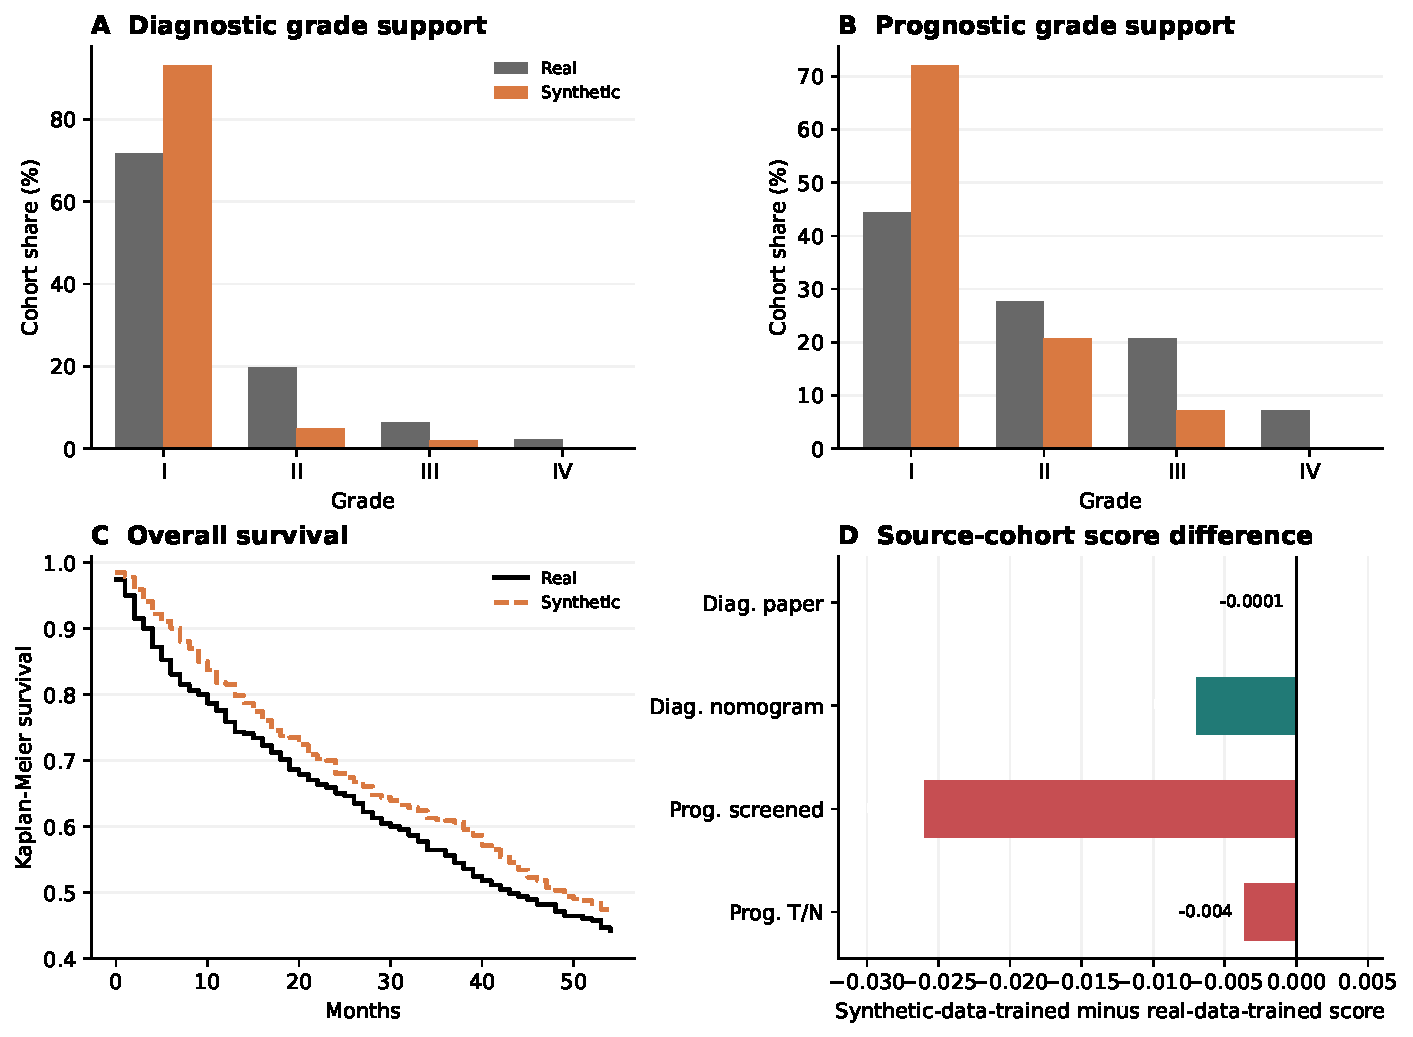
\includegraphics[width=0.88\linewidth]{similarity_fidelity/synthetic_fidelity_summary.pdf}
\caption{Summary of selected fidelity results.  Panels A and B show the
histological-grade distributions, Panel C compares overall Kaplan--Meier
survival and Panel D shows the change in source-cohort discrimination when each
model is trained on synthetic rather than real data.}
\label{fig:fidelity:synthetic}
\end{figure}
\FloatBarrier

These model comparisons are optimistic because the generator was trained on the
same real cohort used for scoring.  The real-data-trained reference models were
also fitted and scored on that complete cohort.  Small differences therefore
show that the modelling procedures can produce similar rankings within the
source data; they do not demonstrate performance at another institution or
preservation of clinical effects.

\subsection{Integrated interpretation and transition}

The results show partial rather than complete preservation.  The TabPFN
embeddings retain substantial local structure and moderate overall distance
ordering, although those findings depend on outcome-inclusive clinical
distances and numerical category coding.  The synthetic cohorts reproduce many
continuous-variable distributions, average correlations and overall survival
features, and some synthetic-trained models retain similar discrimination on
the real source cohort.

Important discrepancies remain.  Statistical discriminators separate real and
synthetic records, grade is strongly distorted, grade IV disappears, several
subgroup survival curves and adjusted relationships change, and 39 of 88 planned
interaction terms cannot be estimated in both cohorts.  The synthetic cohorts
are therefore suitable for testing whether modelling procedures can run and for
carefully qualified exploratory analyses.  They should not replace the real
cohort when interpreting rare categories, regression coefficients, interactions
or clinical survival effects.  The next section broadens the predictive
comparison to additional tabular foundation models while retaining these
evaluation limits.
